\documentclass[a4paper,12pt]{article}

\usepackage{rotating}
\usepackage[top=1in, bottom=1in, left=0.5in, right=0.5in]{geometry}
\usepackage{graphicx}
\usepackage[numbers,square,sort&compress]{natbib}
\usepackage{setspace}
\usepackage[cdot,mediumqspace,]{SIunits}
\usepackage{caption}
\usepackage{subcaption}
\usepackage{mathtools}
\usepackage{authblk}
\usepackage{float}
\renewcommand{\thesubsection}{\thesection.\alph{subsection}}
\providecommand{\e}[1]{\ensuremath{\times 10^{#1}}}

\begin{document}
\onehalfspacing
\title{APM 346 Problem Set 1}
\author{Natalie Price-Jones, 999091021}
\date{September 26 2014}
\affil{\small{natalie.price.jones@mail.utoronto.ca}}
\maketitle

\section{Question 1}

Classify and solve:

\begin{equation}
xu_x - yu_y = 0 \Longleftrightarrow u_x - \frac{y}{x}u_y = 0\nonumber
\end{equation}

The above is true as long as $x\neq$ 0, which we assume. 

Classification: \fbox{first order, linear, homogeneous PDE}

We can rewrite it as: $(1,-\frac{y}{x})\cdot\nabla u = 0$, and we can find a general solution for it with the methods of characteristics. This modified form of the equation makes it obvious that $u$ is constant on curves $\gamma$ with the property $\frac{d}{dt}(x(t),y(t)) = (1,-\frac{y(t)}{x(t)})$. This set of two ODEs is easy to solve, and we find $x(t) = t,\,y(t) = \frac{C}{t} = \frac{C}{x(t)}$, where $C$ is a constant of integration (see below for solution for $y(t)$).

\begin{eqnarray}
\frac{dy(t)}{dt} &=& -\frac{y(t)}{x(t)}\nonumber\\
\frac{dy(t)}{dt} &=& -\frac{y(t)}{t}\nonumber\\
\frac{dy(t)}{y(t)} &=& -\frac{dt}{t}\nonumber\\
y(t) &=& \frac{C}{t}\nonumber
\end{eqnarray}

So $u(x,y)$ is constant on $\gamma = (x,\frac{C}{x})$ by $\frac{d}{dx}u(\gamma(x)) = \frac{d}{dx}u(x,y(x)) = (1,-\frac{y}{x})\cdot\nabla u = 0$. And if $u(x,\frac{C}{x})$ is constant everywhere on the curve, it is constant for $x = 1$

\begin{eqnarray}
u(x,\frac{C}{x}) = const = u(1,C)\nonumber
\end{eqnarray}

So $u$ depends only on $C$, which we can express as $C = xy$, $\implies \boxed{u(x,y) = f(xy)}$. In general, $u$ is some function that depends only on the product of $x$ and $y$.

\section{Question 2}

Classify and find general solution for:

\begin{eqnarray}
au_x + bu_y + cu + d = 0\nonumber
\end{eqnarray}

For $a,b,c,d$ all constant.

Classification: \fbox{first order, linear, inhomogenenous PDE}

As usual, use the method of characteristics. It is useful to rearrange the PDE as follows:

\begin{eqnarray}
u_x + \frac{b}{a}u_y = -\frac{c}{a}u - \frac{d}{a}\nonumber
\end{eqnarray}

The lefthand side can be written $(1,\frac{b}{a})\cdot\nabla u$, and so we want to find the curve $(x,y(x))$ that satisfies $\frac{d}{dx}(x,y(x)) = (1,\frac{b}{a})$. Obviously, we want $y(x) = \frac{b}{a}x + c_1$. With this choice for $y(x)$, our PDE becomes the following ODE:

\begin{eqnarray}
\frac{d}{dx}u(x,y(x)) + \frac{c}{a}u(x,y(x)) = - \frac{d}{a}\label{eqn:ode}
\end{eqnarray}

which we can solve using the method of integrating factors. For simplicity, we define $U(x) = u(x,y(x))$, and try to find $\mu(x)$ such that $\frac{d}{dx}(\mu(x)U(x)) = \mu(x)\frac{d}{dx}U(x) + \frac{c}{a}\mu(x)U(x)$. This looks like the product rule - what we really want is $\mu(x)$ such that $\frac{d}{dx}\mu(x) = \frac{c}{a}\mu(x)$, which implies $\mu(x) = e^{cx/a}$. Multiplying Equation \ref{eqn:ode} by this $\mu$, we find:

\begin{eqnarray}
\mu\frac{d}{dx}U(x) + \mu\frac{c}{a}U(x)= \frac{d}{dx}(\mu U(x))&=& - \frac{d}{a}\mu\nonumber\\
d(e^{cx/a}U(x)) &=& -\frac{d}{a}e^{cx/a} dx\nonumber\\
e^{cx/a}U(x) &=& -\frac{d}{c}e^{cx/a} + c_2\nonumber\\
U(x) = u(x,y(x)) &=& -\frac{d}{c} + c_2 e^{cx/a}
\label{eqn:u}
\end{eqnarray}

Now take Equation ~\ref{eqn:u} at $x = 0$, since we know the behaviour of $y(x)$ at $x = 0$ ($y(0) = c_1$).

\begin{eqnarray}
u(0,y(0)) &=& -\frac{d}{c} + c_2\nonumber\\
\mathrm{However\;we\;can\;rewrite\,} u(0,y(0) &=& u(0,c_1) = f(c_1)\nonumber\\
f(c_1) &=& -\frac{d}{c} + c_2\nonumber\\
\mathrm{We\;also\;know\,} c_1 &=& y-\frac{b}{a}x\nonumber\\
\implies f(c_1) &=& f(y-\frac{b}{a}x) = -\frac{d}{c} + c_2\nonumber\\
\implies c_2 &=& f(y-\frac{b}{a}x) + \frac{d}{c}
\label{eqn:c2}
\end{eqnarray}

So substitute Equation \ref{eqn:c2} into Equation \ref{eqn:u}:

\begin{eqnarray}
u(x,y(x)) = -\frac{d}{c} + (f(y-\frac{b}{a}x) + \frac{d}{c})e^{-cx/a}\nonumber
\end{eqnarray}

The general solution to the PDE is: $\boxed{u(x,y(x)) = -\frac{d}{c} + (f(y-\frac{b}{a}x) + \frac{d}{c})e^{-cx/a}}$

\section{Question 3}

Classify and determine well-posedness of BVP:

\begin{eqnarray}
\left\{
\begin{array}{lr}
u_t + u_x = 0 : x^2 + t^2 < 1\\
u(t,x) = x \mathrm{\,for\,} x^2 + t^2 = 1
\end{array}\right\nonumber
\end{eqnarray}

Classification: \fbox{first order, linear, homogeneous PDE, subject to Dirichlet boundary condition}

As we saw in class, this class of PDE has a general solution $u(t,x) = f(at - bx)$, where for this problem, $a = 1,\ b = 1$. So the boundary condition gives us $u(t,x) = f(t-x) = x$ on $x^2 + t^2 = 1$. Let's think about what we know about $u$ in the $(t,x)$ plane. The figure below shows the characteristic curves (dashed lines), and location of the boundary condition of $u$ (circle).

\begin{figure}[H]
\centering
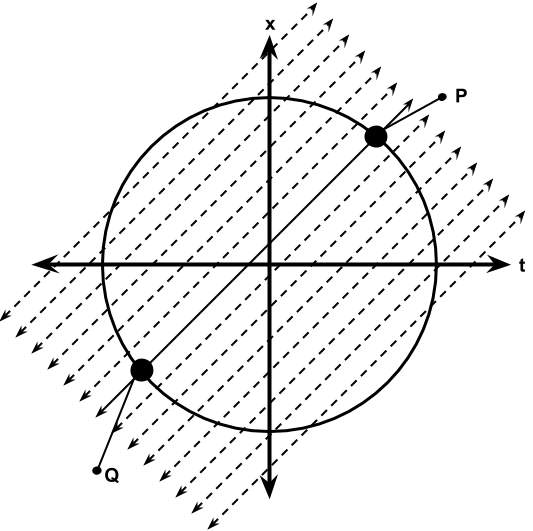
\includegraphics[width = 0.5\linewidth]{APMPS1Q3.png}
\label{fig:q1}
\end{figure}

We choose $P = (t_P,x_P)$ and $Q = (t_Q,x_Q)$ to be points that are both on the boundary and on the same characteristic curve. We know from our PDE that $u(t_P,x_P) = u(t_Q,x_Q) = const$. But our boundary conditions tell us that $u(t_P,x_P) = x_P$ and $u(t_Q,x_Q) = x_Q$. It is obvious from the picture that $x_P\neq x_Q$, and in fact, there are no choices for $P,\,Q$ such that they both lie on the same characteristic curve and satisfy the boundary condition. \fbox{The BVP is not well posed} because there is no way to satisfy the boundary condition. 

\section{Question 4}

Classify and determine well-posedness of BVP:

\begin{eqnarray}
\left\{
\begin{array}{lr}
u_t + u_x = 0\\
u(t=x,x) = 1
\end{array}\right\nonumber
\end{eqnarray}

Classification: \fbox{first order, linear, homogeneous PDE, subject to Dirichlet boundary condition}

This PDE is the same as Question 3, so has the same general solution. The boundary condition is now: $u(t=x,x) = f(x-x) = f(0) = 1$. As with Question 3, we consider the characteristic curves and the BVP. In this case, the general solution gives us that the characteristic curves look like $x = t + C$. Our boundary condition constrains what happens on the curve $x = t$, which is just the characteristic curve where $C = 0$. The boundary condition tells us that $u(t,x)$ is constant on the curve, but our PDE already tells us this. Crucially, the boundary value reveals nothing about the behaviour of $u$ perpendicular to the characteristic curves, so \fbox{the BVP is not well posed}.

\section{Question 5}

Use the method of characteristics to solve:

\begin{eqnarray}
\left\{
\begin{array}{lr}
u_x + yu_y + zu_z = 0\\
u(0,y,z) = y^2 + z^2
\end{array}\right\nonumber
\end{eqnarray}

As usual, we can rewrite our PDE in terms of $\nabla u$

\begin{eqnarray}
u_x + yu_y + zu_z = 0 \Longleftrightarrow (1,y,z)\cdot\nabla u = 0\nonumber
\end{eqnarray}

This makes it obvious that $u$ is constant on curves $\gamma$ with the property: 
\begin{eqnarray}
\frac{d}{dt}\gamma = \frac{d}{dt}(x(t),y(t),z(t)) = (1,y(t),z(t))\nonumber
\end{eqnarray}

This set of three ODEs is easy to solve, providing 

\begin{eqnarray}
\label{eqn:x}
x(t) = t\\
\label{eqn:y}
y(t) = Ce^t = Ce^{x(t)}\\
\label{eqn:z}
z(t) = De^t = De^{x(t)}
\end{eqnarray}

where $C,\,D$ are constants of integration. So $u(x,Ce^x,De^x) = const$, and if this is true, then $u(x,Ce^x,De^x) = u(0,C,D)$. So changes in $u$ depend only on $C$ and $D$. Thus we can write:

\begin{eqnarray}
u(x,y,z) = f(C,D) = f(ye^{-x},ze^{-x})\nonumber
\end{eqnarray}

by rearranging Equations \ref{eqn:y} and \ref{eqn:z} for $C$ and $D$ respectively.

We can determine $f$ with the boundary condition:

\begin{eqnarray}
u(0,y,z) = f(y,z) = y^2+z^2\implies f(ye^{-x},ze^{-x}) = e^{-2x}(y^2 + z^2)\nonumber
\end{eqnarray}

Final answer: $\boxed{u(x,y,z) = e^{-2x}(y^2 + z^2)}$

\section{Question 6}

Classify the following PDE and determine whether it is elliptic, parabolic or hyperbolic. Change variables and reduce the PDE so it's principal part takes the canonical form. Then find constant $\alpha,\,\beta$ such that $u(\xi,\eta) = e^{\alpha\xi + \beta\eta}v(\xi,\eta)$ eliminates the first derivative terms.

\begin{eqnarray}
u_{xx} + 4u_{xy} + 3u_{yy} + 3u_x - u_y + u = 0 
\label{eqn:pde}
\end{eqnarray}

Classification: \fbox{second order, linear, constant coefficient homogeneous partial differential equation}

Calculate discrimnant ($d$) to further determine type:

\begin{eqnarray}
d &=& AC - B^2,\mathrm{\, where\, for\, the\, above\, PDE,\, } A = 1, B = 2, C = 3\nonumber\\
d &=& (1)(3) - 4 < 0\nonumber
\end{eqnarray}

A discriminant less than zero means the \fbox{PDE is hyperbolic}.

This means we want a change of variables such that principal part of the PDE takes the form: $u_{xx} - u_{yy}$. We change from ($x,\,y$) to ($\xi,\,\eta$).

\begin{eqnarray}
\xi &=& ax + by\nonumber\\
\eta &=& cx + dy\nonumber\\
\label{eqn:px}
\partial_x &=& a\partial_{\xi} + c\partial_{\eta}\\
\partial_y &=& b\partial_{\xi} + d\partial_{\eta}
\label{eqn:py}
\end{eqnarray}

Substitute Equations \ref{eqn:px} and \ref{eqn:py} into Equation \ref{eqn:pde} to make the change of variables. Thus our PDE becomes:

\begin{eqnarray}
(a\partial_{\xi} + c\partial_{\eta})^2u &+& 4(a\partial_{\xi} + c\partial_{\eta})(b\partial_{\xi} + d\partial_{\eta})u + 3(b\partial_{\xi} + d\partial_{\eta})^2u\nonumber\\ &+& 3(a\partial_{\xi} + c\partial_{\eta})u - (b\partial_{\xi} + d\partial_{\eta})u + u = 0\nonumber
\end{eqnarray}

Multiply through by $C^2$ to get the slightly nicer form and expand the multiplication terms:

\begin{eqnarray}
(a^2\partial_{\xi}^2 + 2ac\partial_{\xi\eta} + c^2\partial_{\eta}^2)u &+& (4ab\partial_{\xi}^2 + 4ad\partial_{\xi\eta} + 4bc\partial_{\xi\eta} + 4cd\partial_{\eta}^2)u + (3b^2\partial_{\xi}^2 + 6bd\partial_{\xi\eta} + 3d^2\partial_{\eta}^2)u\nonumber\\ &+& 3(a\partial_{\xi} + c\partial_{\eta})u - (b\partial_{\xi} + d\partial_{\eta})u + u = 0\nonumber
\nonumber\\
(a^2 + 4ab + 3b^2)\partial_{\xi}^2u &+& (2ac+4ad+4bc+6bd)\partial_{\xi\eta}u + (c^2 + 4cd + 3d^2)\partial_{\eta}^2u\nonumber\\
&+& (3a-b)\partial_{\xi}u + (3c - d)\partial_{\eta}u + u = 0\nonumber
\end{eqnarray}

The principal part ($pr$, the part we want to reduce to a hyperbolic form) is the first line of the PDE above, and for now this is the only part we will concern ourselves with for the continuing algebra.

\begin{eqnarray}
pr = (a^2 + 4ab + 3b^2)\partial_{\xi}^2u &+& (2ac+4ad+4bc+6bd)\partial_{\xi\eta}u + (c^2 + 4cd + 3d^2)\partial_{\eta}^2u\nonumber
\end{eqnarray}

To put this in hyperbolic form, use the fact that $\partial_{\xi}^2 - m\partial_{\eta}^2$ ($m$ a constant), is still hyperbolic. Thus if $m = g/h$ ($h\neq0$), $h\partial_{\xi}^2 - g\partial_{\eta}^2$ is also hyperbolic. So the only conditions we have on our constants are as follows: 

\begin{eqnarray}
0 &>& a^2 + 4ab + 3b^2 \label{eqn:p1}\\
0 &=& 2ac + 4ad + 4bc + 6bd \label{eqn:p3}\\
0 &<& c^2 + 4cd + 3d^2 \label{eqn:p2}
\end{eqnarray}

Start with Equation \ref{eqn:p2}, and set the right hand side equal to $f(c,d)$. Right away we know that $c$ or $d$, must be less than zero. Since $d$ is an arbitrary constant, set $d = -D$. The easiest way to ensure $f(c,d) < 0$ is to find its minima by setting its partial derivatives with respect to $c$ and $c$ equal to zero.

\begin{eqnarray}
\frac{\partial f}{\partial c} &=& 2c - 4D = 0\nonumber\\
\frac{\partial f}{\partial d} &=& -4c + 6D = 0 \nonumber\\
\implies -4c + 6D &=& 2c - 4D\nonumber\\
c &=& \frac{5}{3}D\label{eqn:ab}
\end{eqnarray}

A quick check shows that if $c$ is given by Equation \ref{eqn:ab}, then $f(c,D) = $$(\frac{25}{9} - \frac{60}{9} + \frac{27}{9})D^2$ $= -\frac{8}{9}D^2 < 0$ for $D$ real.

So choose $D = 3, \implies c = 5$, and so our original $d = -3$. Now find $a$ and $b$ such that Equation \ref{eqn:p3} is satisfied.

\begin{eqnarray}
0 =  10a - 12a + 20b - 18b\implies a = b \nonumber
\end{eqnarray}

Choose $a = 1,\implies b = 1$. Now ensure that the inequality in Equation \ref{eqn:p1} is satisfied: $a^2 + 4ab + 3b^2$ $= 1 + 4 + 3 > 0$. So the final set of constants to make the linear change of coordinates: $a = 1$, $b = 1$, $c = 5$, $d = -3$. We can now rewrite Equation \ref{eqn:pde} as:

\begin{eqnarray}
8u_{\xi\xi} - 8u_{\eta\eta} + 2u_{\xi} + 18u_{\eta} + u = 0\label{eqn:rpde}
\end{eqnarray}

So with the principal part in a canonical form, Equation \ref{eqn:pde} is: $\boxed{8u_{\xi\xi} - 8u_{\eta\eta} + 2u_{\xi} + 18u_{\eta} + u = 0}$

Now, attempt to find $\alpha,\,\beta$ for $u(\xi,\eta) = e^{\alpha\xi - \beta\eta}v(\xi,\eta)$ such that the first-derivative terms in Equation \ref{eqn:rpde} are eliminated. Start by setting $\tau =\tau(\xi,\eta)= \alpha\xi - \beta\eta$ and taking appropriate derivatives of $u$.

\begin{eqnarray}
u_{\xi} &=& \alpha e^{\tau}v + e^{\tau}v_{\xi}\nonumber\\
u_{\eta} &=& \beta e^{\tau}v + e^{\tau}v_{\eta}\nonumber\\
u_{\xi\xi} &=& \alpha^2e^{\tau}v + 2\alpha e^{\tau}v_{\xi} + e^{\tau}v_{\xi\xi}\nonumber\\
u_{\eta\eta} &=& \beta^2e^{\tau}v + 2\beta e^{\tau}v_{\eta} + e^{\tau}v_{\eta\eta}\nonumber
\end{eqnarray}

Substitute the above expressions for derivatives of $u$ into Equation \ref{eqn:rpde} and divide through by $e^{\tau}$

\begin{eqnarray}
8(\alpha^2v + 2\alpha v_{\xi} + v_{\xi\xi}) - 8(\beta^2v + 2\beta v_{\eta} + v_{\eta\eta}) + 2(\alpha v + v_{\xi}) + 18(\beta v + v_{\eta}) + v &=& 0\nonumber\\
8v_{\xi\xi} - 8v_{\eta\eta} + (16\alpha + 2)v_{\xi} + (-16\beta + 18)v_{\eta} + (8\alpha^2 - 8\beta^2 + 2\alpha + 18\beta + 1)v &=& 0\nonumber\\
v_{\xi\xi} - v_{\eta\eta} + 11v &=& 0\nonumber
\end{eqnarray}

Where the last line follows if one chooses $\boxed{\alpha = -1/8,\,\beta = 9/8}$ to eliminate the first derivative terms.
\end{document}